\documentclass[../main.tex]{subfiles}

\begin{document}
	\subsection{W and L sizing influence}
	{
		\begin{tcolorbox}[colback=gray!5!white,colframe=gray!75!black]
			We select a charge capacitance of $0,5pF$.
			\begin{itemize}
				\item Measure the variation of the propagation times when the resistance of the N transistor is decreased by increasing $W_n$. Plot the graph $T_p^{\text{up} \to \text{down}}(W_n)$.
				\item Measure the variation of the propagation times when the resistance of the N transistor is decreased by increasing $W_n$. Plot the graph $T_p^{\text{down} \to \text{up}}(W_p)$.
			\end{itemize}
		\end{tcolorbox}
		
		\subsubsection{$T_p(\text{up} \to \text{down})$ function of $W_n$}
		{
			
			The values of $W_n$ chosen for simulation and measurement were: $2\mu m$, $3\mu m$, $6\mu m$, $9\mu m$, $12\mu m$. I tried $W_n = 1\mu m$ but for low values of $W_n$, the output does not even reach $\frac{V_{DD}}{2}$.
			
			\begin{table}[htbp]
				\centering
				\renewcommand{\arraystretch}{1.5} % Adjust row height
				\begin{tabular}{|c|c|}
					\hline
					$W_n$ & $T_p(\text{up} \to \text{down})$ \\ \hline
					$2\mu m$ & $2,48ns$  \\ \hline
					$3\mu m$ & $1,69ns$ \\ \hline
					$6\mu m$   & $0,91ns$ \\ \hline
					$9\mu m$   & $0,69ns$ \\ \hline
					$12\mu m$   & $0,56ns$ \\ \hline
				\end{tabular}
				\caption{Propagation time measured for each value of $W_n$}
				\label{tab:wndep}
			\end{table}
			
			\begin{figure}[H]
				\centering
				% Subfigure 1
				\begin{subfigure}{0.3\textwidth}
					\centering
					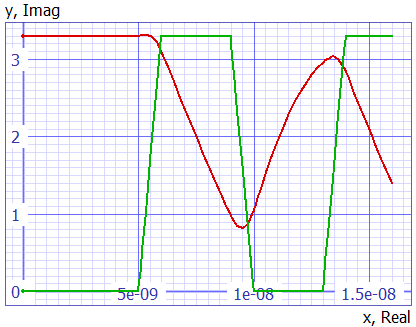
\includegraphics[width=\textwidth]{plots/Q7_Wn2.png}
					\caption{$W_n = 2\mu m$}
					\label{fig:subfig1}
				\end{subfigure}
				% Subfigure 2
				\begin{subfigure}{0.3\textwidth}
					\centering
					\includegraphics[width=\textwidth]{plots/Q6_05pf.png}
					\caption{$W_n = 3\mp m$}
					\label{fig:subfig2}
				\end{subfigure}
				% Subfigure 3
				\begin{subfigure}{0.3\textwidth}
					\centering
					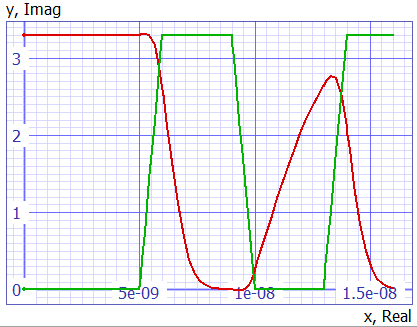
\includegraphics[width=\textwidth]{plots/Q7_Wn6.png}
					\caption{$W_n = 6\mu m$}
					\label{fig:subfig3}
				\end{subfigure}
				
				% Subfigure 4
				\begin{subfigure}{0.3\textwidth}
					\centering
					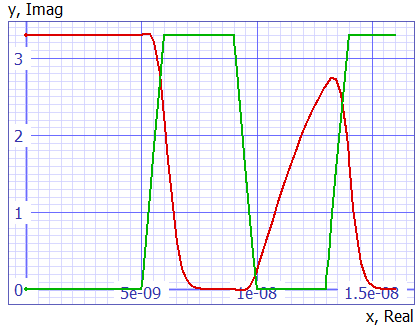
\includegraphics[width=\textwidth]{plots/Q7_Wn9.png}
					\caption{$W_n = 9\mu m$}
					\label{fig:subfig4}
				\end{subfigure}
				% Subfigure 5
				\begin{subfigure}{0.3\textwidth}
					\centering
					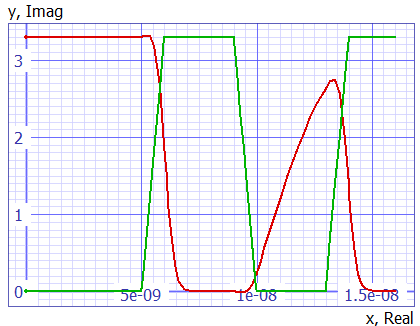
\includegraphics[width=\textwidth]{plots/Q7_Wn12.png}
					\caption{$W_n = 12\mu m$}
					\label{fig:subfig5}
				\end{subfigure}
				
				\caption{Output \textcolor{red}{$V_{out}$ in red} and input \textcolor{green}{$V_{in}$ in green} for different values of $W_n$}
				\label{fig:mainfigWn}
			\end{figure}
			
			When we plot $T_p(\text{up} \to \text{down})$ as a function of $W_n$, we observe that $T_p(\text{up} \to \text{down})$ seems to decrease exponentially and for large values of $W_n$ it approaches some constant. Therefore, the appropriate fit is
			$$T_p^{\text{up} \to \text{down}}(W_n) = a\cdot e^{-bW_n} + c$$
			
			\begin{figure}[H]
				\centering
				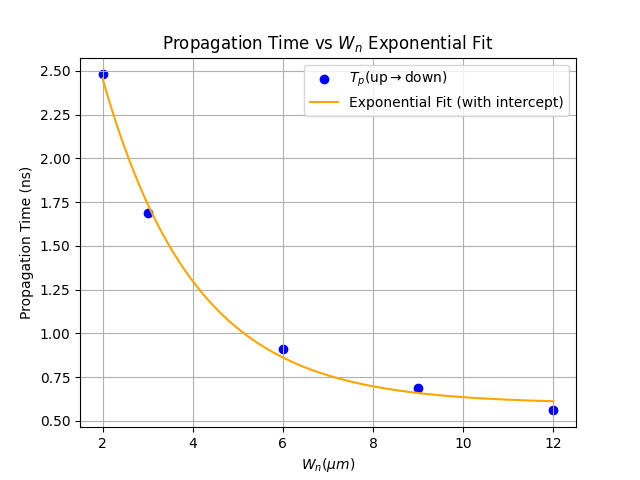
\includegraphics[width=0.5\textwidth]{plots/Q7_Wn_plot.png}
				\caption{Propagation time $T_p(\text{up} \to \text{down})$ as function of $W_n$}
			\end{figure}
			
			
		}
		
		\subsubsection{$T_p(\text{down} \to \text{up})$ function of $W_p$}
		{
			The values of $W_p$ chosen for simulation and measurement were: $4\mu m$, $5\mu m$, $6\mu m$, $9\mu m$, $12\mu m$. I tried $W_p = 3\mu m$ but similarly to what we verified for $W_n$, for low values of $W_p$, the output does not even reach $\frac{V_{DD}}{2}$.
			
			\begin{table}[htbp]
				\centering
				\renewcommand{\arraystretch}{1.5} % Adjust row height
				\begin{tabular}{|c|c|}
					\hline
					$W_p$ & $T_p(\text{down} \to \text{up})$ \\ \hline
					$4\mu m$ & $2,82ns$  \\ \hline
					$5\mu m$ & $2,22$ \\ \hline
					$6\mu m$ & $1,81ns$ \\ \hline
					$9\mu m$ & $1,31ns$ \\ \hline
					$12\mu m$& $1,01ns$ \\ \hline
				\end{tabular}
				\caption{Propagation time measured for each value of $W_p$}
				\label{tab:wpdep}
			\end{table}
			
			\begin{figure}[H]
				\centering
				% Subfigure 1
				\begin{subfigure}{0.3\textwidth}
					\centering
					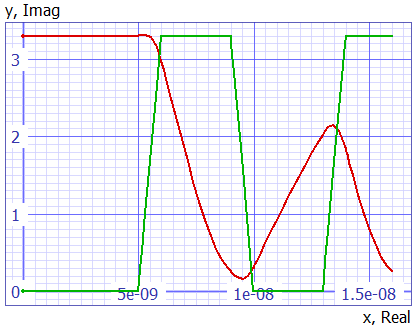
\includegraphics[width=\textwidth]{plots/Q7_Wp4.png}
					\caption{$W_p = 4\mu m$}
					\label{fig:subfig1}
				\end{subfigure}
				% Subfigure 2
				\begin{subfigure}{0.3\textwidth}
					\centering
					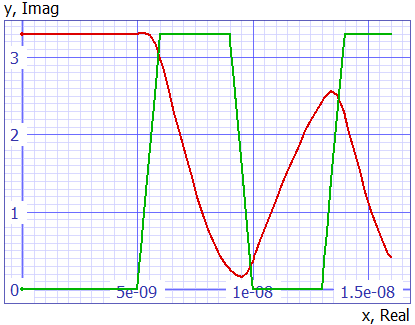
\includegraphics[width=\textwidth]{plots/Q7_Wp5.png}
					\caption{$W_p = 5\mu m$}
					\label{fig:subfig2}
				\end{subfigure}
				% Subfigure 3
				\begin{subfigure}{0.3\textwidth}
					\centering
					\includegraphics[width=\textwidth]{plots/Q6_05pf.png}
					\caption{$W_p = 6\mu m$}
					\label{fig:subfig3}
				\end{subfigure}
				
				% Subfigure 4
				\begin{subfigure}{0.3\textwidth}
					\centering
					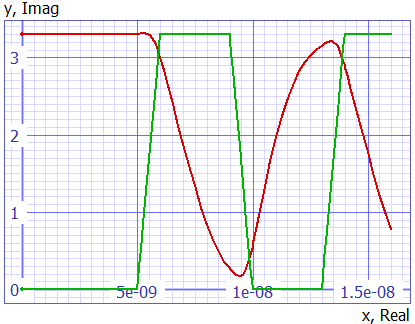
\includegraphics[width=\textwidth]{plots/Q7_Wp9.png}
					\caption{$W_p = 9\mu m$}
					\label{fig:subfig4}
				\end{subfigure}
				% Subfigure 5
				\begin{subfigure}{0.3\textwidth}
					\centering
					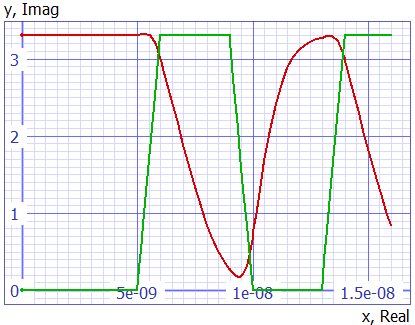
\includegraphics[width=\textwidth]{plots/Q7_Wp12.png}
					\caption{$W_p = 12\mu m$}
					\label{fig:subfig5}
				\end{subfigure}
				
				\caption{Output \textcolor{red}{$V_{out}$ in red} and input \textcolor{green}{$V_{in}$ in green} for different values of $W_p$}
				\label{fig:mainfigWn}
			\end{figure}
			
			Now, when we plot $T_p(\text{down} \to \text{up})$ as a function of $W_p$, we observe that $T_p(\text{down} \to \text{up})$ seems to decrease exponentially and for large values of $W_p$ it approaches some constant. Therefore, the appropriate fit is
			$$T_p^{\text{down} \to \text{up}}(W_p) = a\cdot e^{-bW_p} + c$$
			
			\begin{figure}[H]
				\centering
				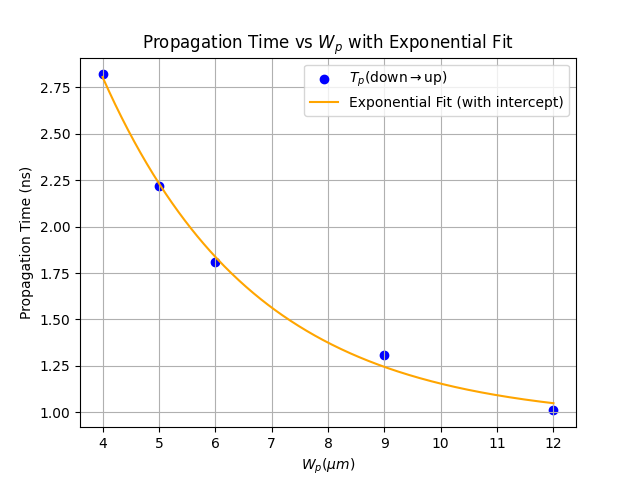
\includegraphics[width=0.5\textwidth]{plots/Q7_Wp_plot.png}
				\caption{Propagation time $T_p(\text{down} \to \text{up})$ as function of $W_p$}
			\end{figure}
			
		}
		
	}
\end{document}